\mainmatter%
\setcounter{page}{1}

\lectureseries[\course]{\course}

\auth[\lecAuth]{Lecturer: \lecAuth\\ Scribe: \scribe}
\date{October 29, 2009}

\setaddress%

% the following hack starts the lecture numbering at 10
\setcounter{lecture}{9}
\setcounter{chapter}{9}

\lecture{Controlled Markov Chains I}

\section{Markov Chains Review}
A Markov chain is defined by $(\mathbb{X},\mathbb{P})$ and has $\dim(\mathbb{X})=N<\infty$.

The probability transition matrix is $\pij=P(\xi_{t+1}=j|\xi_t=i)$.
Recall that $\pij^n={[\mathbb{P}^n]}_{i,j}$.

A distribution $\Pi\in S^N$ is a stationary distribution if $\Pi=\mathbb{P}^T\Pi$.

$(\mathbb{X},\mathbb{P})$ is irreducible if $i\leftrightarrow j~\forall~i,j\in\mathbb{X}$.
This means that the system can get from any state $i$ to any state $j$ with a positive probability.

Some Markov chains exhibit periodicity (oscillation).
If there exists $n>1$ such that $\pij^n>0$ then $d(i)=\text{GCD}(\{n\geq1|\pij^n>0\})$, else $d(i)=0$.
Note that $\text{GCD}$ is the greatest common divisor.
Then, $(\mathbb{X},\mathbb{P})$ is aperiodic if $d(i)=1~\forall~i\in\mathbb{X}$.

Proofs for these can be found in ``Probability Measure'' by Patrick Billingsley for the most part.

\begin{lemma}
If $\mc$ is finite, irreducible and aperiodic then there exists $n_0(i,j)<\infty$ such that $\pij^n>0~\forall~n\geq n_0(i,j)$.
\end{lemma}
Let $\bar{n}_0=\max_{i,j\in\mathbb{X}}n_0(i,j)$, then $\pij^n>0~\forall~i,j\in\mathbb{X},~\forall~n\geq n_0$.
This means that eventually all the probabilities are greater than zero for going from one state to another.

\begin{theorem}
\label{th:distconverge}
If $\mc$ is finite, irreducible and aperiodic then there exists $A\in[0,\infty], \rho\in[0,1)$ and a stationary distribution $\Pi$ such that% chktex 9
$$|\pij^n-\Pi_j|\leq A\rho^n~\forall~n\geq1,~\forall~i,j$$
\end{theorem}
This theorem implies convergence where all the rows of $\mathbb{P}^n$ converge to the distribution $\Pi$.

Let $p_0\in S^N$ and $p_{t+1}=\mathbb{P}^T p_t~\forall~t$.
Then
\begin{align*}
\lim_{t\to\infty}p_{t_j} &= \lim_{t\to\infty}\sum_{i=1}^N\pij^t p_{0_i} = \sum_{i=1}^N\left[\lim_{t\to\infty}\pij^t\right]p_{0_i} \\
&= \sum_{i=1}^N\Pi_j p_{0_i} = \Pi_j\underbrace{\sum_{i=1}^N p_{0_i}}_{=0} = \Pi_j
\end{align*}
This shows convergence $p_t\rightarrow\Pi$ is independent of $p_0$.

To see that $\Pi$ is unique if it is a stationary distribution we have
$$\mathbb{P}^T\hat{\Pi} = \hat{\Pi} \Rightarrow {(\mathbb{P}^T)}^2\hat{\Pi} = \hat{\Pi} \Rightarrow \cdots$$
So, if $p_0=\hat{\Pi}$ then $p_t=\hat{\Pi}~\forall~t$, but $p_t\rightarrow\Pi \therefore \hat{\Pi}=\Pi$.

\begin{corollary}
If $\mc$ is finite, irreducible and aperiodic then $p_t\rightarrow\Pi$ for any $p_0\in S^N$.
Further, there exists a unique solution to $\Pi=\mathbb{P}^T\Pi \in S^N$.
\end{corollary}
This means there is only one eigenvector for $\lambda=1$.

\begin{example}
Let
$$\mathbb{P} = \left[\begin{array}{c c} 0 & 1 \\ 1 & 0 \end{array}\right]$$
Then $\mathbb{P}^2=I \Rightarrow~\mathbb{P}^{2n+1}=\mathbb{P}, \mathbb{P}^{2n}=I~\forall~n$.
This leads to
\begin{align*}
p_0 = \left[\begin{array}{c} q \\ 1-q \end{array}\right],
\qquad p_1 = \left[\begin{array}{c} 1-q \\ q \end{array}\right],
\qquad p_2 = p_0,
\qquad p_3=p_1,\ldots
\end{align*}
See Figure~\ref{fig:10mc2}.
$\lozenge$
\end{example}

\begin{figure}[ht!]
\centering
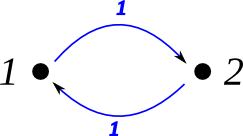
\includegraphics[width=.4\textwidth]{images/10mc2}
\caption{Two state Markov chain.}
\label{fig:10mc2}
\end{figure}

\begin{example}
Let
$$\mathbb{P} = \left[\begin{array}{c c c} 1 & 0 & 0 \\ \frac{1}{3} & \frac{1}{3} & \frac{1}{3} \\ 0 & 0 & 1 \end{array}\right]$$
Then $d (1)=d (2)=d (3)=1$ means the system is aperiodic.
Also, it is not irreducible as seen from $1\nrightarrow~3$, $3\nrightarrow~2$ and $1\nrightarrow~2$.
Then $p_0=\left[\begin{array}{c c c} q & 0 & 1-q \end{array}\right]^T \Rightarrow~p_t=p_0~\forall~t$.
See Figure~\ref{fig:10mc3a}.
$\lozenge$
\end{example}

\begin{figure}[ht!]
\centering
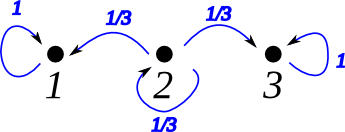
\includegraphics[width=.4\textwidth]{images/10mc3a}
\caption{Three state Markov chain.}
\label{fig:10mc3a}
\end{figure}

\begin{example}
Let
$$\mathbb{P} = \left[\begin{array}{c c c} \frac{1}{2} & \frac{1}{2} & 0 \\ 0 & 0 & 1 \\ \frac{1}{2} & \frac{1}{2} & 0 \end{array}\right]$$
From Figure~\ref{fig:10mc3b} we can see that $1\leftrightarrow~3$, $1\leftrightarrow~2$ and $2\leftrightarrow~3$ meaning that the system is irreducible.
Also, $d (1)=1$ so by Theorem~\ref{th:periodicity} about equivalence classes it must be true that $d (2)=d (3)=d (1)=1$ and the system is aperiodic.
Let
\begin{align*}
p_0 &= \left[\begin{array}{c} 0 \\ 0 \\ 1 \end{array}\right],
\qquad p_1 = \mathbb{P}^Tp_0 = \left[\begin{array}{c} \frac{1}{2} \\ \frac{1}{2} \\ 0 \end{array}\right], \\
p_2 = \mathbb{P}^Tp_1 &= \left[\begin{array}{c} \frac{1}{4} \\ \frac{1}{4} \\ \frac{1}{2} \end{array}\right],
\qquad p_3 = \mathbb{P}^Tp_2 = \left[\begin{array}{c} \frac{3}{8} \\ \frac{3}{8} \\ \frac{1}{4} \end{array}\right]
\end{align*}
Next we can look for the eigenvector corresponding to $\lambda=1$.
\begin{align*}
&(\mathbb{P}^T-I)\Pi = 0 \\
&\left[\begin{array}{c c c} -\frac{1}{2} & 0 & \frac{1}{2} \\ \frac{1}{2} & -1 & \frac{1}{2} \\ 0 & 1 & -1 \end{array}\right]
\left[\begin{array}{c} \pi_1 \\ \pi_2 \\ \pi_3 \end{array}\right] = 0 \\
&\Rightarrow~\pi_1=\pi_3, \qquad \pi_2=\pi_3 \qquad \Rightarrow~\Pi=\left[\begin{array}{c} \frac{1}{3} \\ \frac{1}{3} \\ \frac{1}{3} \end{array}\right]
\end{align*}
The system should converge to $\Pi$ relatively quickly, $\sim\frac{1}{N}$.
$\lozenge$
\end{example}

\begin{figure}[ht!]
\centering
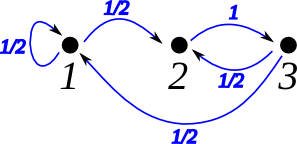
\includegraphics[width=.4\textwidth]{images/10mc3b}
\caption{Three state Markov chain.}
\label{fig:10mc3b}
\end{figure}

\begin{example}
\label{ex:gambling}
Let's look at the gambling example again.
Let the player start with $\$x$ and the house with $\$y$.
We have $\mathbb{X}=\]1,N\[$ and $N=x+y+1$.% chktex 10
The initial condition is $\xi_0=x+1$.
The player wins with probability $p$ and loses with probability $q=1-p$.
The probability transistion matrix is given by
$$\mathbb{P} = \left[\begin{array}{c c c c c} 1 & 0 & 0 & 0 & 0 \\ q & 0 & p & 0 & 0 \\ 0 & q & 0 & p & 0 \\ 0 & 0 & q & 0 & p \\ 0 & 0 & 0 & 0 & 1 \end{array}\right]$$
Looking at the eigenspace we can see that
\begin{align*}
&(\mathbb{P}^T-I) = \left[\begin{array}{c c c c c} 0 & q & 0 & 0 & 0 \\ 0 & -1 & q & 0 & 0 \\ 0 & p & -1 & q & 0 \\ 0 & 0 & p & -1 & 0 \\ 0 & 0 & 0 & p & 0 \end{array}\right] \\
& (\mathbb{P}^T-I) = 0
\end{align*}
From this we see that
\begin{align*}
&q\pi_2 = 0 \Rightarrow \pi_2=0 \\
&-\pi_2+q\pi_3 = 0 \Rightarrow \pi_3=0 \\
&\vdots \\
&\Rightarrow \Pi = \left[\begin{array}{c} \beta \\ 0 \\ 0 \\ 0 \\ 1-\beta \end{array}\right]
\end{align*}
where $\beta\in[0,1]$.
This $\Pi$ is not unique because Theorem~\ref{th:distconverge} does not hold.
It can be seen that $p_t\rightarrow \Pi(p_0)\in\mathcal{N}\cap S^N$.
Then let
$$p_{0_i}(j) = \begin{cases} 1, & i=j \\ 0, & i\neq j \end{cases}$$
This corresponds to the player starting with $\$j-1$.
Then
$$p_t(j) = {(\mathbb{P}^t)}^T p_0(j) \rightarrow \Pi(j)\in\mathcal{N}$$
We can define the payoff for $\xi_0=j$ to be
\begin{align*}
J(j) &= \lim_{T\to\infty}E[\xi_T-1] = \lim_{T\to\infty}\sum_{i=1}^N (i-1)p_{t_i}(j) \\
&= \sum_{i=1}^N (i-1)\lim_{T\to\infty} p_{t_i}(j) = \sum_{i=1}^N (i-1) \Pi_i(j) \\
&= 0\cdot \Pi_1(j) + (N-1)\Pi_N(j) = (N-1)\Pi_N(j)
\end{align*}
Suppose instead that the rules state the maximum bet is set such that neither the player nor the house can end up in negative territory.
If $\xi_t=j$ then the maximum bet is $\min\{j-1,N-j\}$ is our policy.
To construct $\mathbb{P}$ for that policy at least one of the ends will be non-zero.
Then the payoff can be determined and can be compared to the original gambling policy and payoff.
$\lozenge$
\end{example}

\section{Controlled Markov Chains}
Given $\pij=\pij(u)$ with $u\in\mathcal{U}$ the feedback $u$ knows the state $i$.
$$\mathcal{M}=\{\mu:\mathbb{X}\rightarrow\mathcal{U}\}$$
If $\mathcal{U}$ is finite then $\text{size}(\mathcal{M})=\text{size}(\mathcal{U})$.
This means that there a finite number of control policies to explore and can greatly simplify control problems.
Another bit of notation is that given $\mu\in\mathcal{M}$, let $\pij^\mu \doteq \pij(\mu(i))$.

\begin{example}
Consider a setting with two UAVs.
Let $\mathbb{X}=\{1,2,3\}$ where state $1$ is both UAVs are inoperational, state $2$ is one UAV inoperational and one UAV operational while state $3$ means both UAVs are operational.
Our control space consists of $\mathcal{U} = \{A,B,C\}$ where $A$ means fly all operational UAVs, $B$ means fly $\min\{1, \#\text{operational}\}$ (or fly one UAV if there are any that are operational, else don't fly any UAVs) and $C$ means fly all operational UAVs and repair all inoperational UAVs.
Let the probability transition matrices be
\begin{align*}
\begin{split}
\mathbb{P}(A) = \left[\begin{array}{c c c} 1 & 0 & 0 \\ \frac{1}{2} & \frac{1}{2} & 0 \\ \frac{1}{4} & \frac{1}{2} & \frac{1}{4} \end{array}\right],
\mathbb{P} (B) = \left[\begin{array}{c c c} 1 & 0 & 0 \\ \frac{1}{2} & \frac{1}{2} & 0 \\ 0 & \frac{1}{2} & \frac{1}{2} \end{array}\right],
\mathbb{P} (C) = \left[\begin{array}{c c c} \frac{2}{5} & \frac{2}{5} & \frac{1}{5} \\ \frac{1}{4} & \frac{1}{2} & 0 \\ \frac{1}{4} & \frac{1}{2} & \frac{1}{4} \end{array}\right]
\end{split}
\end{align*}
We get the control policies as
$$\mu(i) = \begin{cases} C, & i=1 \\ A, & i=2 \\ B, & i=3 \end{cases}$$
This allows us to build up the probability transition matrix corresponding to the control policy as
$$\mathbb{P}^\mu = \left[\begin{array}{c c c} \frac{2}{5} & \frac{2}{5} & \frac{1}{5} \\ \frac{1}{2} & \frac{1}{2} & 0 \\ 0 & \frac{1}{2} & \frac{1}{2} \end{array}\right]$$
It can be seen that $\mathbb{P}^\mu$ is built up using the first row of $\mathbb{P} (C)$, the second row of $\mathbb{P} (A)$ and the third row of $\mathbb{P} (B)$ according to the control policy, $\mu(i)$, since $\pij^\mu=\pij(\mu(i))$.

For the running cost we can use infinite time horizon because we don't know how long these missions will continue, so $l (i,u)=l_1(i)+l_2(u)$.
Then the discounted cost, infinite time horizon payoff is
$$J (j,\mu) = \lim_{T\to\infty}E\left[\sum_{t=0}^T \alpha^t l (\xi_t,\mu(\xi_t))\right]$$
Since $\text{size} (\mathcal{M})<\infty$ we can use minimize the value function using
$$V (j) = \min_{\mu\in\mathcal{M}}J (j,\mu)$$
The next steps are to prove the Dynamic Programming Principle (DPP) for one-step ahead in order to find the Dynamic Programming Equation (DPE).
The DPE should look like
\begin{align*}
V(j) &= \min_{u\in\mathcal{U}}\left\lbrace l(i,u)+\alpha E[V(\xi)]\right\rbrace \\
&= \min_{u\in\mathcal{U}}\left\lbrace l(j,u) + \alpha \sum_{i=1}^N\left[V(i)\pji\right]\right\rbrace
\end{align*}
where we used $\xi_0=j$ in the second equality.
Then we have $V=\mathcal{G}[V]$ and this lets us proceed to using value iteration to solve for $V$.
$\lozenge$
\end{example}% chktex 17
